\documentclass[12pt,letterpaper]{exam}
\usepackage[lmargin=1in,rmargin=1in,tmargin=1in,bmargin=1in]{geometry}
\usepackage{../style/exams}

% -------------------
% Course & Exam Information
% -------------------
\newcommand{\course}{MATH 122: Final Exam}
\newcommand{\term}{Fall --- 2024}
\newcommand{\examdate}{12/10/2024}
\newcommand{\timelimit}{150 Minutes}

\setbool{hideans}{false} % Student: True; Instructor: False

% -------------------
% Content
% -------------------
\begin{document}

\examtitle
\instructions{Write your name on the appropriate line on the exam cover sheet. This exam contains \numpages\ pages (including this cover page) and \numquestions\ questions. Check that you have every page of the exam. Answer the questions in the spaces provided on the question sheets. Be sure to answer every part of each question and show all your work. If you run out of room for an answer, continue on the back of the page --- being sure to indicate the problem number.} 
\scores
\bottomline
\newpage

% Poem
\phantom{.} \vfill
	\begin{table}[h]
	\centering
	\begin{tabular}{l}
	{\itshape 'Twas the night before Christmas, up at the Pole,} \\
	{\itshape Santa was frazzled---he'd lost all control!} \\
	{\itshape The reindeer were restless, the sleight off its track,} \\
	{\itshape And the toy distribution? A logistical smack!} \\
	\\
	{\itshape Santa scratched his beard, eyes weary and red,} \\
	{\itshape ``The math here is tricky. I'm in over my head!} \\
	{\itshape The children are waiting, and I need to take flight.} \\
	{\itshape I need a Calculus wizard to save Christmas tonight!''}
	\end{tabular}
	\end{table}
\phantom{.} \vfill 

% -------------------
% Questions
% -------------------
\begin{questions}

% Question 1
\newpage
\question[10] {\itshape Santa’s workshop is busy, the costs start to climb, \par \phantom{(XX points)} ``Help me with this function---I'm running out of time!''} \par\vspace{0.3cm}

The cost to produce toys for a small town for the North Pole toy manufacturing production line is given by $C(q)= 0.01q^2 + 1.7q + 15760$, where $q$ is the number of toys produced and $C$ is measured in dollars. Showing all your work\dots
	\begin{enumerate}[(a)]
	\item Find the cost to produce 3,700 toys. \pspace
	
		\[
		C(3700)= 0.01(3700)^2 + 1.7(3700) + 15760= 136900 + 6290 + 15760= \$158,\!950
		\] \par\vspace{3.3cm}
	
	\item Find the fixed costs to produce the toys for this small town. \pspace
		\[
		C(0)= 0.01(0)^2 + 1.7(0) + 15760= \$15,\!760 
		\]  \pvspace{4cm}
	
	\item Find and interpret the marginal cost to produce 3,700~toys. \pspace
		
		{\itshape
			\[
			\begin{gathered}
			C'(q)= 0.02q + 1.7 \\[0.2cm]
			C'(3700)= 75.7
			\end{gathered}
			\] \pspace
		Therefore, the cost to produce the 3,701st toy is approximately \$75.70. 
		}
	\end{enumerate}



% Question 2
\newpage
\question[10] {\itshape Santa's gifts bring joy, but his budget's not lit, \par \phantom{(XX points)} ``Help me crunch the numbers---I need to make a profit!''} \par\vspace{0.3cm}

To help produce enough toys during the year, Santa has Bernard the Elf sell snow globes. Each snow globe is sold for \$119.99 and costs approximately \$8.34 to produce. However, the costs to maintain the North Pole snow globe manufacturing plant are huge---approximately \$250 million. Showing all your work, find the minimal number of snow globes Santa needs to sell to turn a profit. \pspace

{\itshape \tsol Each globe sells for \$119.99, which makes the revenue function $R(q)= 119.99q$. The variable costs are $8.34q$ because each snow globe costs \$8.34 to produce. The fixed costs are \$250~million. Therefore, the cost function is $C(q)= 8.34q + 250000000$. The breakeven point occurs when revenue equals cost. We have\dots
	\[
	\begin{gathered}
	R(q)= C(q) \\[0.3cm]
	119.99q= 8.34q + 250000000 \\[0.3cm]
	111.65q= 250000000 \\[0.3cm]
	q\approx 2,\!239,\!140.17
	\end{gathered}
	\]
Therefore, Bernard would have to sell at least 2,239141 snow globes to turn a profit for Santa. 
}



% Question 3
\newpage
\question[10] {\itshape Santa's sleigh is in peril, the night's looking rough, \par \phantom{(XX points)} ``Help me read this graph---Christmas math is tough!''} \par\vspace{0.3cm}

Consider the {\bfseries plot of a function $f(x)$} shown below. 
	\[
	\fbox{
	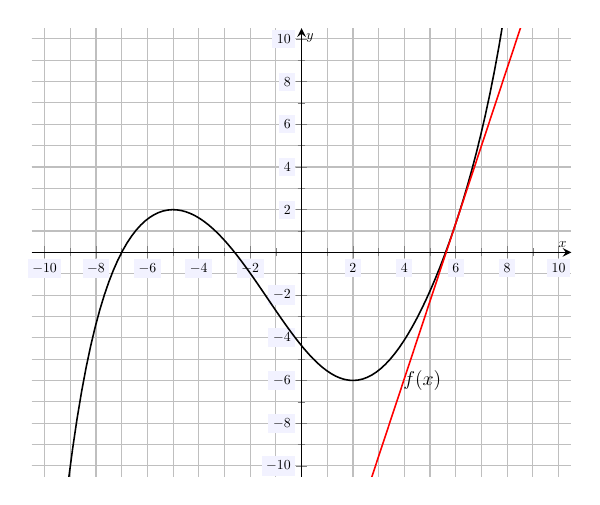
\begin{tikzpicture}[scale=1,every node/.style={scale=0.5}]
	\begin{axis}[
	grid=both,
	axis lines=middle,
	ticklabel style={fill=blue!5!white},
	xmin= -10.5, xmax=10.5,
	ymin= -10.5, ymax=10.5,
	xtick={-10,-8,-6,-4,-2,0,2,4,6,8,10},
	ytick={-10,-8,-6,-4,-2,0,2,4,6,8,10},
	minor tick = {-10,-9,...,10},
	xlabel=\(x\),ylabel=\(y\),
	]
	\addplot[line width= 0.02cm,samples=120,domain= -10.5:10.5] ({x},{-4.37348 - 1.46973*x + 0.231455*x^2 + 0.0556307*x^3 - 0.00249594*x^4 - 0.000614528*x^5 + 0.0000156713*x^6 + 0.00000528689*x^7});
	\node at (4.7,-6) {\Large$f(x)$};
	\addplot[line width= 0.02cm,samples=4,domain= -10.5:10.5,red] ({x},{3.63503*x - 20.4556});
	\end{axis}
	\end{tikzpicture}
	}
	\] 
Based on the plot above, answer the following: \par
	\begin{enumerate}[(a)]
        	\item On what interval(s)---if any---is $f'(x) > 0$? \vfill
		\[
		(-\infty, -5) \cup (2, \infty)
		\] \vfill
	
	\item On what interval(s)---if any---is $f'(x) < 0$? \vfill
		\[
		(-5, 2)
		\] \vfill
	
	\item Find the critical values---if any---for $f(x)$. \vfill
		\[
		x= -5, \,\, 2
		\] \vfill
	
	\item Find the points of inflection---if any---for $f(x)$. \vfill
		\[
		x= -1.3
		\] \vfill
	
	\item On what interval(s)---if any---is $f''(x) > 0$? \vfill
		\[
		(-1.3, \infty)
		\] \vfill
	
	\item On what interval(s)---if any---is $f''(x) < 0$? \vfill
		\[
		(-\infty, -1.3)
		\] \vfill
	
	\item Sketch the tangent line to $f(x)$ at $x= 6$ on the graph above. \vfill
	\end{enumerate}



% Question 4
\newpage
\question[10] {\itshape Santa's old graph was flawed, it led him astray, \par \phantom{(XX points)} ``Help me solve this new one, or Christmas won't stay!''} \par\vspace{0.3cm}

Consider the {\bfseries plot of a derivative $f'(x)$} shown below. {\bfseries This is not the graph of the function, $f(x)$.}
	\[
	\fbox{
	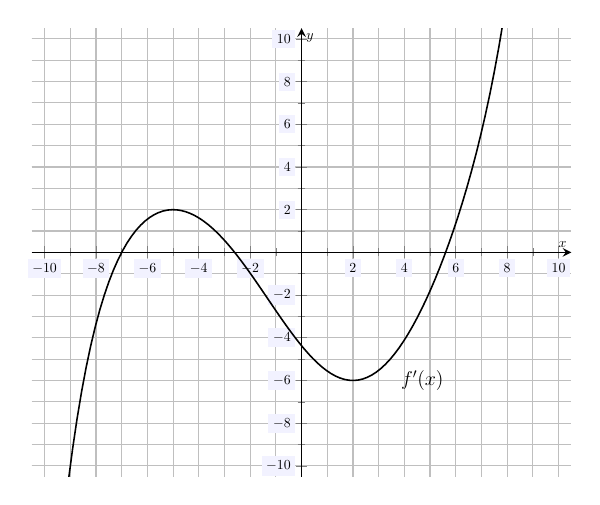
\begin{tikzpicture}[scale=1,every node/.style={scale=0.5}]
	\begin{axis}[
	grid=both,
	axis lines=middle,
	ticklabel style={fill=blue!5!white},
	xmin= -10.5, xmax=10.5,
	ymin= -10.5, ymax=10.5,
	xtick={-10,-8,-6,-4,-2,0,2,4,6,8,10},
	ytick={-10,-8,-6,-4,-2,0,2,4,6,8,10},
	minor tick = {-10,-9,...,10},
	xlabel=\(x\),ylabel=\(y\),
	]
	\addplot[line width= 0.02cm,samples=120,domain= -10.5:10.5] ({x},{-4.37348 - 1.46973*x + 0.231455*x^2 + 0.0556307*x^3 - 0.00249594*x^4 - 0.000614528*x^5 + 0.0000156713*x^6 + 0.00000528689*x^7});
	\node at (4.7,-6) {\Large$f'(x)$};
	\end{axis}
	\end{tikzpicture}
	}
	\] 
Based on the plot above, answer the following questions: 
	\begin{enumerate}[(a)]
	\item On what interval(s)---if any---is $f(x)$ increasing? \vfill
		\[
		(-7, -2.6) \cup (5.6, \infty)
		\] \vfill
	
	\item On what interval(s)---if any---is $f(x)$ decreasing? \vfill
		\[
		(-\infty, -7) \cup (-2.6, 5.6)
		\] \vfill
	
	\item On what interval(s)---if any---is $f(x)$ concave up? \vfill
		\[
		(-\infty, -5) \cup (2, \infty)
		\] \vfill
	
	\item On what interval(s)---if any---is $f(x)$ concave down? \vfill
		\[
		(-5, 2)
		\] \vfill
	
	\item Find any critical values for $f(x)$---if any. \vfill
		\[
		x= -7, \,\, -2.6, \,\, 5.6
		\] \vfill
	
	\item Classify any critical values you found in (e). \vfill
		\[
		\text{Local Min} \colon x= -7, 5.6 \qquad \text{Local Max} \colon x= -2.6
		\] \vfill
	
	\item Find any points of inflection for $f(x)$. \vfill
		\[
		x= -5, \,\, 2
		\] \vfill
	\end{enumerate}



% Question 5
\newpage
\question[10] {\itshape Santa's sleigh's gone off course, the math isn't quite right, \par \phantom{(XX) points)} ``Quick, help me compute these derivatives this Christmas night!''} \par\vspace{0.3cm}

Showing all your work, compute the following derivatives: \par\vspace{0.3cm}
	\begin{enumerate}[(a)]
	\item $\dfrac{d}{dx} \left( \dfrac{\sqrt[3]{\pi^2} \ln(15)}{19^{-3}} \right)= 0$ \vfill
	\item $\dfrac{d}{dx} \left( 4x^3 - 5^x + \sqrt[3]{x} \right)= \dfrac{d}{dx} \left( 4x^3 - 5^x + x^{1/3} \right)= 12x^2 - 5^x \ln 5 + \dfrac{1}{3}\, x^{-2/3}$ \vfill
	\item $\dfrac{d}{dx} \left( (x^2 - 7) e^x \right)= 2x e^x + (x^2 - 7) e^x$ \vfill
	\item $\dfrac{d}{dx} \ln(5x^2 - 9)= \dfrac{1}{5x^2 - 9} \cdot 10x$ \vfill
	\item $\dfrac{d}{dx} \left( \dfrac{3x^4}{x^2 - x} \right)= \dfrac{12x^3 (x^2 - x) - (2x - 1)3x^4}{(x^2 - x)^2}$ 
	\end{enumerate}



% Question 6
\newpage
\question[10] {\itshape Santa's sleigh is tilting, the path's tough to find, \par \phantom{(XX points)} ``Help me with the tangent---Christmas is on the line!''} \par\vspace{0.3cm}

Consider the function $f(x)= x^2 - 6x + 4$. Showing all your work\dots
	\begin{enumerate}[(a)]
	\item Find the tangent line to $f(x)$ at $x= -2$. \pspace
	
		{\itshape We find the derivative to find the slope.
			\[
			\begin{aligned}
			f'(x)&= 2x - 6 \\
			f'(-2)&= 2(-2) - 6= -4 - 6= -10 
			\end{aligned}
			\]
		Using the fact that $f(-2)= (-2)^2 - 6(-2) + 4= 4 + 12 + 4= 20$, we have the point $(-2, 20)$. Therefore, the tangent line is\dots
			\[
			y= y_0 + m(x - x_0)= 20 + (-10) \big(x - (-2) \big)= 20 - 10(x + 2)
			\]
		} \vspace{3.7cm}
	
	\item Find the absolute maximum and absolute minimum of $f(x)$ on $[0, 8]$. \pspace
	
		{\itshape We have $f'(x)= 2x - 6$. We need to find the critical values, e.g. the values where $f'(x)= 0$. But then $2x - 6= 0$. This implies that $2x= 6$, so that $x= 3$. We can check whether this is a maximum or a minimum using the first derivative test:
			\[
			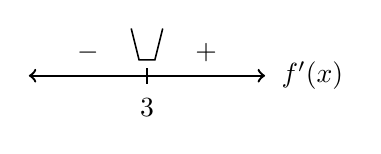
\begin{tikzpicture}
			\draw[line width=0.03cm,<->] (-1.5,0) -- (1.5,0);
			\draw[line width=0.02cm] (0,-0.1) -- (0,0.1);
			\node at (2.1,0) {$f'(x)$};
			\node at (0,-0.4) {$3$};
			\node at (-0.75,0.3) {$-$};
			\node at (0.75,0.3) {$+$};
			\draw[line width=0.02cm] (-0.2,0.6) -- (-0.1,0.2) -- (0.1,0.2) -- (0.2,0.6);
			\end{tikzpicture}
			\]
		Therefore, we can see that $x= 3$ is a local minimum. We compare the value of $f(x)$ at $x= 3$ to its value at the endpoints:
			\[
			\begin{aligned}
			f(3)= 3^2 - 6(3) + 4= 9 - 18 + 4= -5 \\
			f(0)= 0^2 - 6(0) + 4= 0 - 0 + 4= 4 \\
			f(8)= 8^2 - 6(8) + 4= 64 - 48 + 4= 20
			\end{aligned}
			\]
		Therefore, the absolute minimum is $-5$ and occurs at $x= 3$ and the absolute maximum is $20$ and occurs at $x= 8$.
		}
	\end{enumerate}



% Question 7
\newpage
\question[10] {\itshape Santa's sleigh is on point, but his math's in a tizz, \par \phantom{(XX points)} ``Quick, estimate this integral---I can't lose my rizz!''} \par\vspace{0.3cm}

The speed of Santa's sleigh in mph, $v(t)$, at a time $t$ (in hours) as he races across the globe at several different times since the start of Christmas are given in the table below. \par
	\begin{table}[!ht]
	\centering
	\begin{tabular}{|l||c|c|c|c|c|c|c|} \hline
	Time, $t$ & 0 & 2 & 3 & 6 & 7 \\ \hline
	Velocity, $v(t)$ & 844 & 2,440 & 7,640 & 9,330 & 6,210 \\ \hline
	\end{tabular}
	\end{table} \par
Showing all your work and being as accurate as possible, use a left-hand sum to estimate and interpret $\ds\int_0^7 v(t) \;dt$. \pspace

{\itshape \tsol We can create a rough sketch of the left-hand sum:
	\[
	\fbox{
	\pgfplotsset{scaled y ticks=false}
	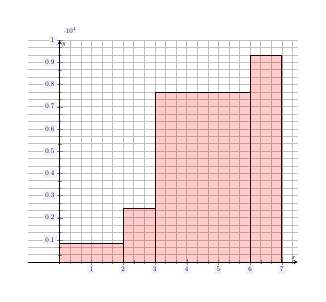
\begin{tikzpicture}[scale=0.5,every node/.style={scale=0.5}]
	\begin{axis}[
	grid=both,
	axis lines=middle,
	ticklabel style={fill=blue!5!white},
	xmin= -1, xmax=7.5,
	ymin= -100, ymax=10000,
	xtick={0,1,2,...,8},
	ytick={0,1000,...,10000},
	minor y tick num= 2,
	minor x tick num=2,
	xlabel=\(x\),ylabel=\(y\),
	]
	\draw[line width=0.02cm] (0,0) -- (2,0) --(2,844) -- (0,844) -- (0,0);
	\draw[fill=red,opacity=0.20] (0,0) -- (2,0) --(2,844) -- (0,844) -- (0,0);
	\draw[line width=0.02cm] (2,0) -- (3,0) --(3,2440) -- (2,2440) -- (2,0);
	\draw[fill=red,opacity=0.20] (2,0) -- (3,0) --(3,2440) -- (2,2440) -- (2,0);
	\draw[line width=0.02cm] (3,0) -- (6,0) -- (6,7640) -- (3,7640) -- (3,0);
	\draw[fill=red,opacity=0.20] (3,0) -- (6,0) -- (6,7640) -- (3,7640) -- (3,0);
	\draw[line width=0.02cm] (6,0) -- (7,0) -- (7,9330) -- (6,9330) -- (6,0);
	\draw[fill=red,opacity=0.20] (6,0) -- (7,0) -- (7,9330) -- (6,9330) -- (6,0);
	\end{axis}
	\end{tikzpicture}
	}
	\]
Computing the total area of these rectangles, we have\dots
		\[
		\int_0^7 v(t) \;dt \approx 2(844) + 1(2440) + 3(7640) + 1(9330)= 1,\!688 + 2,\!440 + 22,\!920 + 9,\!330= 36,\!378
		\]
We know that $\ds\int_0^7 v(t) \;dt$ represents the net change in the distance traveled over the next seven hours. Therefore, Santa has traveled a net distance of 36,378~mi over the past seven hours.
}



% Question 9
\newpage
\question[10] {\itshape Santa's graph is confusing, the numbers don't show, \par \phantom{(XX points)}``Help me compute this integral, so I know where to go!''} \par\vspace{0.3cm}

A function $f(x)$ is plotted below. \par
	\[
	\fbox{
	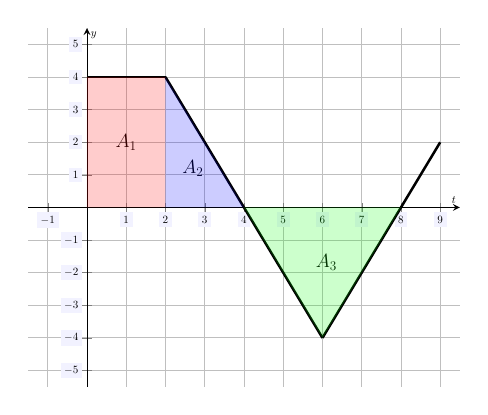
\begin{tikzpicture}[scale=0.8,every node/.style={scale=0.5}]
	\begin{axis}[
	grid=both,
	axis lines=middle,
	ticklabel style= {fill= blue!5!white},
	xmin= -1.5, xmax=9.5,
	ymin= -5.5, ymax=5.5,
	xtick= {-2,-1,...,10},
	ytick= {-6,-5,...,6},
	minor tick = {-10,-9,...,10},
	xlabel= \(t\), ylabel= \(y\)
	]
	\addplot[line width=0.04cm, samples=4, smooth, domain= 0:2] {4};
	\addplot[line width=0.04cm, samples=4, smooth, domain= 2:6] {8 - 2*x};
	\addplot[line width=0.04cm, samples=4, smooth, domain= 6:9] {2*x - 16};
	
	\node at (1,2) {\LARGE$A_1$};
	\node at (2.7,1.2) {\LARGE$A_2$};
	\node at (6.1,-1.7) {\LARGE$A_3$};
	
	\draw[draw=none,fill=red,opacity=0.2] (0,0) -- (2,0) -- (2,4) -- (0,4) -- (0,0);
	\draw[draw=none,fill=blue,opacity=0.2] (2,0) -- (4,0) -- (2,4) -- (2,0);
	\draw[draw=none,fill=green,opacity=0.2] (4,0) -- (6,-4) -- (8,0) -- (4,0);
	\end{axis}
	\end{tikzpicture}
	}
	\] 
Showing all your work, based on the graph above, compute the following: \par\vspace{0.3cm}
	\begin{enumerate}[(a)]
	\item $\ds\int_0^4 f(x) \;dx= A_1 + A_2= 2(4) + \frac{1}{2} (2)4= 8 + 4= 12$ \vfill
	\item $\ds\int_4^8 f(x) \;dx= -A_3= -\frac{1}{2} (4)4= -8$ \vfill
	\item $\ds\int_0^8 f(x) \;dx= A_1 + A_2 - A_3= 8 + 4 - 8= 4$ \vfill
	\item $\ds\int_5^5 f(x) \;dx= 0$ \vfill
	\item The area between $f(x)$ and the $x$-axis. 
		\[
		\text{Area}= A_1 + A_2 + A_3= 8 + 4 + 4= 16
		\] \pvspace{0.3cm}
	\end{enumerate}



% Question 9
\newpage
\question[10] {\itshape Addressing Christmas challenges, Santa has another request. \par \phantom{(XX points)} ``Help me solve this problem---then we'll pass this tough test!''} \par\vspace{0.3cm}
 
 Showing all your work, compute the following: \par\vspace{0.3cm}
 	\begin{enumerate}[(a)]
	\item $\ds\int (x^5 - e^x + 7) \;dx$ \vfill
		\[
		\int (x^5 - e^x + 7) \;dx= \frac{1}{6}\, x^6 - e^x + 7x + C
		\] \vfill
	\item $\ds\int \dfrac{x^6 - x^2 + 9}{x^2} \;dx$ \vfill
		\[
		\int \dfrac{x^6 - x^2 + 9}{x^2} \;dx= \int \left( \dfrac{x^6}{x^2} - \dfrac{x^2}{x^2} + \dfrac{9}{x^2} \right) \;dx= \int \left( x^4 - 1 + 9x^{-2} \right) \;dx= \dfrac{1}{5}\,x^5 - x - 9x^{-1} + C
		\] \vfill
	
	\item $\ds\int_{-1}^3 (4 - 3x^2) \;dx$ \vfill
		\[
		\int_{-1}^3 (4 - 3x^2) \;dx= 4x - x^3 \bigg|_{-1}^3= \big(4(3) - 3^3\big) - \big(4(-1) - (-1)^3 \big)= -15 - (-3)= -12 
		\] \vfill
	\end{enumerate}

 
 
 % Question 10
\newpage
\question[10] {\itshape Christmas almost over, you're nearly clear. \par \phantom{(XX points)} ``Help me find these integrals, then we're done for this year.''} \par\vspace{0.3cm}

Showing all your work, use $u$-substitution to find the following: \par\vspace{0.3cm}
	\begin{enumerate}[(a)]
	\item $\ds\int \dfrac{x}{x^2 + 1} \;dx$ \pspace
	
	{\itshape Making a $u$-substitution, we have\dots \par
	\begin{minipage}[b]{0.3\textwidth}
		\[
		\begin{aligned}
		u&= x^2 + 1 \\
		\\
		du&= 2x \;dx \\
		dx&= \dfrac{1}{2x} \, du
		\\ \\ \\ \\ \\ \\ \\ \\
		\end{aligned}
		\]
	\end{minipage}\begin{minipage}[b]{0.3\textwidth}
		\[
		\begin{gathered}
		\int \dfrac{x}{x^2 + 1} \;dx \\[0.2cm]
		\int \dfrac{x}{u} \cdot \dfrac{1}{2x} \; du \\[0.2cm]
		\int \dfrac{1}{2u} \;du \\[0.2cm]
		\dfrac{1}{2} \int \dfrac{1}{u} \;du \\[0.2cm]
		\dfrac{1}{2} \ln|u| + C \\[0.2cm]
		\dfrac{1}{2} \, \ln|x^2 + 1| + C
		\end{gathered}
		\]
	\end{minipage}
	} \pvspace{1.1cm}
	
	\item $\ds\int_0^1 (1 - 2x)^{10} \;dx$ \pspace

	{\itshape Making the $u$-substitution and changing bounds, we have\dots
		\[
		\begin{aligned}
		u&= 1 - 2x \hspace{1cm}& x=1 &\colon u= 1 - 2(1)= 1 - 2= -1 \\
		du&= -2 \;dx \hspace{1cm}& x= 0 &\colon u= 1 - 2(0)= 1 - 0= 1 \\
		dx&= -\dfrac{1}{2} \, du
		\end{aligned}
		\]

		\[
		\int_0^1 (1 - 2x)^{10} \;dx= \int_1^{-1} u^{10} \cdot -\dfrac{1}{2} \; du= -\dfrac{1}{2} \int_1^{-1} u^{10} \;du= -\dfrac{1}{2} \cdot \dfrac{u^{11}}{11} \bigg|_1^{-1}
		\]
	But then we have\dots
		\[
		-\dfrac{1}{2} \cdot \dfrac{u^{11}}{11} \bigg|_1^{-1}= -\dfrac{1}{22} u^{11} \bigg|_1^{-1}= -\dfrac{1}{22} \cdot \big (-1)^{11} - 1^{11} \big)= -\dfrac{1}{22} \cdot (-1 - 1)= -\dfrac{1}{22} \cdot -2= \dfrac{1}{11} \approx 0.0909
		\]
	}
	\end{enumerate}
\end{questions}

\end{document}